\documentclass[conference]{IEEEtran}
\usepackage{times}

% numbers option provides compact numerical references in the text. 
\usepackage[numbers]{natbib}
\usepackage{multicol}
\usepackage[bookmarks=true]{hyperref}
\usepackage{graphics} % for pdf, bitmapped graphics files
\usepackage{graphicx}
\usepackage{amsmath,amssymb,latexsym,float,epsfig,subfigure}
\usepackage{amsmath} % assumes amsmath package installed
\usepackage{amssymb}  % assumes amsmath package installed
\usepackage{lipsum}
\usepackage[export]{adjustbox}
\usepackage[normalem]{ulem} % underline
\usepackage{wrapfig}
\usepackage{multirow}
\usepackage{balance}
\usepackage{color}
\usepackage{url}
\usepackage{booktabs}
\usepackage{pifont}
\newcommand{\argmax}{\arg\!\max}
\newcommand{\norm}[1]{\left\lVert#1\right\rVert}
\pdfinfo{
   /Author (Deepak Gopinath, Brenna D. Argall)
   /Title  (Mode Switch Assistance to Human Intent Disambiguation)
   /CreationDate (January 31 2017)
   /Subject (Robots)
   /Keywords (Robots)
}

\begin{document}

% paper title
\title{Mode Switch Assistance to\\Maximize Human Intent Disambiguation}
%\author{Author Names Omitted for Anonymous Review. Paper-ID [\textbf{163}]}
% You will get a Paper-ID when submitting a pdf file to the conference system
%\author{Deepak Gopinath and Brenna D. Argall}

%\author{\authorblockN{Deepak Gopinath}
%\authorblockA{Department of Mechanical\\Engineering,
%Northwestern University\\
%Evanston, Illinois 30332\\
%Email: deepakedakkattilgopinath2015\\@u.northwestern.edu}
%\and
%\authorblockN{Brenna D. Argall}
%\authorblockA{Department of Mechanical\\Engineering,
%		Northwestern University\\
%		Evanston, Illinois 30332\\
%		Email: brenna.argall@northwestern.edu}
%	}

%\author{Deepak Gopinath$^{1}$ and Brenna D. Argall$^{2}$
%	\thanks{Manuscript received: March, 1, 2016; Revised June,
%		7, 2016; Accepted June, 29, 2016.}
%}
% avoiding spaces at the end of the author lines is not a problem with
% conference papers because we don't use \thanks or \IEEEmembership


% for over three affiliations, or if they all won't fit within the width
% of the page, use this alternative format:
% 
\author{\authorblockN{Deepak E. Gopinath\authorrefmark{1}\authorrefmark{2},
Brenna D. Argall\authorrefmark{1}\authorrefmark{2}\authorrefmark{3}\authorrefmark{4}
}
\authorblockA{
	\authorrefmark{1}Department of Mechanical Engineering, Northwestern University, Evanston, IL}

\authorblockA{\authorrefmark{2}Rehabilitation Institute of Chicago, Chicago, IL}

\authorblockA{\authorrefmark{3}Department of Physical Medicine and Rehabilitation, Northwestern University, Chicago, IL}

\authorblockA{\authorrefmark{4}Department of Electrical Engineering and Computer Science, Northwestern University, Evanston, IL}

\authorblockA{{\tt\small deepakgopinath@u.northwestern.edu}}
\authorblockA{{\tt\small brenna.argall@northwestern.edu}}
}


\maketitle

\begin{abstract}

In this paper, we develop an algorithm for intent inference via goal disambiguation with a shared-control assistive robotic arm. Assistive systems are often required to infer human intent and this \textcolor{blue}{often is} a bottleneck for providing assistance quickly and accurately. We introduce the notion of \textit{inverse legibility} in which the human-generated actions are legible enough for the \textit{robot} to infer the human intent confidently and accurately. The proposed disambiguation paradigm seeks to elicit legible control commands from the human by selecting control modes \textcolor{blue}{for the robotic arm in which human-directed motion will} \textit{maximally disambiguate} between \textcolor{blue}{multiple} goals. We present simulation results which look into the robustness of our algorithm and the impact of the choice of confidence functions on the performance of the system. 
%Our simulation results suggest that the disambiguating control mode computed by our algorithm produces more intuitive results when the confidence function is able to capture the ``directedness'' towards a goal. 
Our simulations results suggest that the choice of confidence function is a critical factor in determining the disambiguation algorithm's capability to capture human intent. We also present a pilot study that explores the efficacy of the algorithm on real hardware with promising preliminary results.
% indicate that the assistance paradigm proposed \textcolor{blue}{is a promising approach} in decreasing task effort (number of mode switches) across interfaces and tasks. 
\end{abstract}

\IEEEpeerreviewmaketitle

\section{Introduction}

Assistive and rehabilitation devices such as powered wheelchairs, robotic arms and myoelectric prostheses play an important role in the lives of people with motor impairments. These devices help to increase \textcolor{blue}{the human's} ability to perform activities of daily lives and reduce their dependence on caretakers, and are crucial to revolutionizing the way people with motor impairments interact with society. As the field of assistive robotics progresses rapidly, the devices themselves become more capable and dextrous---and as a result also more complex, higher dimensional and harder to control. 

\textcolor{blue}{To operate an assistive device, typically} the human directly control\textcolor{blue}{s} the device motion via a control interface. However, the more severe a person's motor impairment, the more limited are the control interfaces available for them to use. These interfaces (for example, a switch-based head array or Sip-N-Puff) are lower in dimensionality and bandwidth, and \textcolor{blue}{generally are able to operate on only a subset of the device control space at a given time}. Therefore, we have a difficult situation, in which sophisticated assistive devices that require complex control strategies are paired with users with diminished ability to control them.
%Thus, a greater need for sophisticated assistive devices is paired with a diminishing ability to control their additional complexity. 

Due to the mismatch between the dimensionality of the control interface and controllable degrees-of-freedom (D\textcolor{blue}{o}F) of the robotic device, control interfaces typically operate in \textit{modes} which correspond to different partitions of the control space. By necessity, the more limited the control interface is, the greater number of modes there are. In order to have full control of the robot the user will have to switch between the different partitions and this is known as \textit{mode switching} or \textit{modal control}~\cite{nuttin2002selection,tsui2008development}. 

It has been established that mode switching is expensive and as a result task performance is degraded~\cite{herlant2016assistive}. Furthermore, it adds to the cognitive and physical burden \textcolor{blue}{of the human} as each of these mode switches requires the user to shift their attention from the task to performing the mode switch. The introduction of \textit{shared autonomy} to these systems helps to alleviate and address some of these issues by letting the system take partial responsibility of \textcolor{blue}{the} task execution, thereby reducing the human effort in achieving a goal. 
%\begin{wrapfigure}[12]{R}{0.25\textwidth}
\begin{figure}[b]
	\begin{center}
%		\vspace{-0.8cm}
		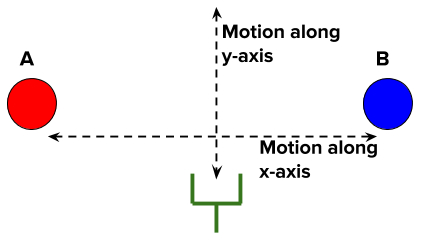
\includegraphics[width=0.285\textwidth]{./figures/DE_NEW3.png}
	\end{center}
%	\vspace{-.45cm}
	\caption{Illustration of goal disambiguation along various control dimensions. Any motion of the end effector (green) along the y-axis will not help the system to disambiguate the two goals (A and B). However, motion along the x-axis provides cues as to which goal.}
	\label{DE}
\end{figure}

%\begin{figure}
%	%	\centering
%	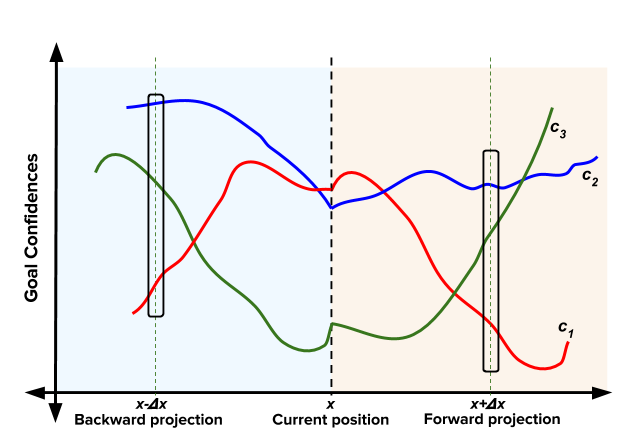
\includegraphics[width = 1\hsize, height = 0.26\vsize]{./figures/DisambMetric_New2.png}
%	\vspace{-0.4cm}
%	\caption{Illustration of change in confidence with movement along a single control dimension. A very different distribution of confidences results from positive motion (beige) versus negative motion (blue). Snapshots after moving by amount $\Delta x$ highlighted by rectangles.}
%	\label{DM_FIG}
%\end{figure}
 Any assistive autonomy system typically needs an idea of what it is the human is trying to do---either by explicit indication from the user of the task or goal~\cite{choi2008laser}, or by inferring the human's intent from their control signals or sensor data~\cite{tavakkoli2007vision,wasson2003user}. The question of intent inference \textcolor{blue}{thus} is key. In this paper, we develop an assistance paradigm that helps with intent inference, by selecting the control mode in which robot motion will \textit{maximally disambiguate} human intent. The faster the autonomy is able to disambiguate intent, the earlier the robot is able to provide autonomy assistance---leading ideally to fewer mode switches and less burdensome executions. 


Within the field of Human-Robot Interaction (HRI) a \textit{legible} motion is one which helps the observer (usually the human) decipher the intent behind the robot's action more \textit{quickly} and \textit{confidently}~\cite{dragan2013legibility}. It can be the case that certain actions \textit{by the human} might carry more information about the human's intent---which can then help the robot to draw useful and correct inferences more easily. Therefore, in this paper we propose a paradigm of \textit{inverse legibility} in which the roles are switched and the human-generated actions \textit{help the robot} to infer human intent confidently and accurately. 
%\textbf{[Can there be a concept of bilateral legibility? The human knows the goal. And therefore has a model for what a predictable motion is. If the robot indeed performs that predictable motion, there is an agreement between the expectation and what really happened. That is, the robot motion becomes legible.]}

Consider the example illustrated in Figure~\ref{DE}. A human control command issued along the $x$ dimension is more \textit{intent expressive} and helps the robot to provide \textcolor{blue}{appropriate} assistance \textcolor{blue}{more} quickly and confidently. With the disambiguation assistance scheme developed in this work, we hope to elicit more legible \textit{human} control commands by placing the user control in those modes that \textit{maximally disambiguate} between the various goals in the scene. 


In Section \ref{RW} we present an overview of relevant research in the area of shared control in assistance systems focusing on mode switching, legibility and synergies in HRI. Section \ref{ALGO} describes the mathematical formalism for the algorithm and the metric used for goal disambiguation, \textcolor{blue}{and Section~\ref{IMPL} describes the details of our implementation}. The simulation results are presented in Section~\ref{SIMRESULTS}, and the pilot study in Section \ref{EXP}. Conclusions are provided in Section \ref{DC}.

\section{RELATED WORK}\label{RW} 

This section provides a brief overview of related research in the areas of intent inference, robot assistance for modal control, legibility and cooperation in HRI.

Shared-control assistance paradigms help to offload cognitive and physical burden~\cite{volosyak2005rehabilitation} without requiring the user to relinquish complete control, and are usually preferred over fully autonomous assistive robotic systems for reasons of both robustness and user satisfaction. Often, shared control systems require an estimate of the human's intent---their intended task, goal or motion, for example. Methods for intent inference have been extensively studied by roboticists and cognitive scientists alike and can be broadly classified into two categories: model-based and heuristic-based~\cite{baker2017rational}. In model-based approaches the agent is typically modeled as a Partially Observable Markov Decision Process (POMDP) that acts according to a policy that maps states to actions. In such settings, intent inference reduces to solving the inverse problem of computing the posterior distribution over mental states conditioned on observed actions (Bayesian Inference)~\cite{baker2007goal,baker2009action}. Heuristic-based approaches instead seek to find direct mappings between some signals---such as low-level motion cues~\cite{barrett2005accurate} or biological signals~\cite{donoghue2002connecting}---and the underlying human intention. Our approach builds on a heuristic-based intent inference framework. More specifically, we use a \textit{confidence function} as a measure of the robot's estimate that a particular goal is indeed the user's intended goal. Confidence functions typically depend on the human control command, autonomous policy, robot pose or goal locations, and often are used to dictate how much control lies with the robot versus with the human in the shared-control system. 
% One possible way to control high-dimensional assistive devices such as robotic arms is to partition the control space (often 6D for a robotic arm) into subsets called \textit{modes} and have the user control one mode at a time using control interfaces such as joysticks, head arrays and sip-and-puffs. This is known as \textit{modal control}.

The cognitive burden of shifting focus (\textit{task switching}) from the task at hand to mode switch\textcolor{blue}{ing} can result in a significant decrease in task performance regardless of the control modality~\cite{monsell2003task}. \textcolor{blue}{Users in many cases find} \textit{modal control} and \textit{mode switching} to be slow, difficult \textcolor{blue}{or} burdensome~\cite{herlant2016assistive}. Even a simple time-optimal automatic mode switching system can significantly improve user satisfaction while maintaining quality task performance~\cite{herlant2016assistive}. \textcolor{blue}{However, also} it is not always the case that users are trying to optimize for time or effort during task execution~\cite{gopinath2017human}. Our present system therefore does not make \textit{a priori} assumptions regarding the optimizing principles at work when a user operates a robot.

The legibility and predictability of robot motion \textit{to the human} \textcolor{blue}{is} thoroughly investigated~\cite{dragan2013legibility}, and different methods for generating legible robot motion \textcolor{blue}{are} proposed~\cite{holladay2014legible}. We apply this concept of legibility however to the \textit{human control} commands, such that the intent expressed in the human command is clear \textit{to the robot}. \textcolor{blue}{We term this \textit{inverse legibility}}. Our assistance scheme is intended to bring out a more legible intent-expressive control command from the human, by placing the user control in that mode which can provide maximal goal disambiguation and improved legibility.

Eliciting legible commands from the user can also be thought of as an information acquisition problem. Information acquisition in robotic systems  have been widely studied, primarily in the context of generating optimal control for mobile robot sensing systems. A typical approach is to model the problem as an optimal control problem with an associated reward structure that reflects some measure of information gain~\cite{atanasov2014information}. The problem of information gathering \textcolor{blue}{for example can be} formulated as maximizing the ergodicity of a robot's trajectory with respect to an underlying information density map~\cite{miller2013trajectory,miller2016ergodic} by evaluating the expected value of the Fisher information---the amount of information a single measurement reveals at a location. 
%In most cases the human knows beforehand what goal he/she is going for and therefore the motion generated by the human is usually \textit{predictable}.


Also related to our work is the idea of mutual cooperation between humans and robots, and the underlying synergies that are crucial for successful human-robot interaction. In order to overcome the communication bottleneck that exists between robots and people during human-robot interactions, different types of user interfaces have been developed \textcolor{blue}{that} account for the constrained capabilities of the robot~\cite{goodfellow2010help}. A framework for \textit{``people helping robots helping people''} \textcolor{blue}{has} humans provide semantic information and judgments about the environment to the robot, which then utilizes them to improve its own capabilities~\cite{sorokin2010people}. A \textit{symbiotic} human robot interaction scheme aims to overcome perceptual and cognitive limitations that robots might encounter while still allowing the robots to help humans~\cite{rosenthal2010effective}. From the robot's perspective the key concept behind our algorithm is the idea of \textit{``Help Me, Help You''}---that is, if the human can ``help'' the robot by providing more legible control commands, then the robot in turn can assist the human more quickly and effectively.

\begin{figure}
%	\centering
	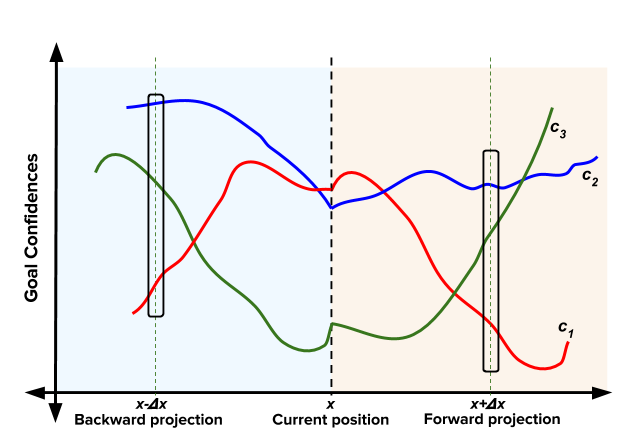
\includegraphics[width = 1\hsize, height = 0.26\vsize]{./figures/DisambMetric_New2.png}
	\vspace{-0.4cm}
	\caption{Illustration of change in confidence with movement along a single control dimension. A very different distribution of confidences results from positive motion (beige) versus negative motion (blue). Snapshots after moving by amount $\Delta x$ highlighted by rectangles.}
	\label{DM_FIG}
\end{figure}
\section{ALGORITHM DESIGN} \label{ALGO}
This section describes our algorithm that computes the control mode that is \textcolor{blue}{able to maximally disambiguate between human goals}, thereby eliciting the most legible control command from the human. Section~\ref{NOT} outlines the mathematical notation used in the paper and Section~\ref{DM} describes the formulation and computation of the metric used to disambiguate human intent. 

\subsection{Notation}\label{NOT}

Let $\mathcal{G}$ be the set of all candidate user goals with $n_g = \vert\mathcal{G}\vert$ and let $g^{i}$ refer to the $i^{th}$ goal where $i \in [1,2,\dots,n_g]$. A \textit{goal} represents the intent of the human, and might be a task or location in the world, for example. The set of goals corresponds to an associated set of confidences denoted as $\mathcal{C}$, where $c^{i}$ refers to the individual confidence associated with goal $g^{i}$---that is, the robot's confidence that $g^{i}$ represents the human's intent. Let $\mathcal{K}$ be the control space in which the robot operates and $k^{i}$ refer to an individual control dimension where $i \in [1,2,\dots,n_k]$.  The cardinality of $\mathcal{K}$ depends on the robotic platform; for example, for a smart wheelchair $n_k = 2$ whereas for a six degrees-of-freedom robotic arm $n_k = 6$.

For control purposes, the set $\mathcal{K}$ is partitioned into subsets known as \textit{modes}. Let $\mathcal{M}$ refer to the set of all modes that the control space $\mathcal{K}$ is partitioned into with $n_{m} = \vert\mathcal{M}\vert$. The number of modes $n_{m}$ is specific to the control interface and mapping to $\mathcal{K}$. Furthermore, let $m^{i}$ refer to the $i^{th}$ mode where $i \in [1,2,\dots,n_{m}]$.

Another quantity of interest is the spatial gradient of individual goal confidences for motions along the various control dimensions. More specifically, the gradient \textcolor{blue}{is} denoted by $\frac{\partial c}{\partial x_k}$, where $c \in \mathcal{C}$ and $x_k$ is the component of robot's position along control dimension $k$. Furthermore, since the confidence function in general can assume drastically different values upon moving in positive and negative directions within a given control dimension, the positive and negative gradients are explicitly denoted as $\frac{\partial c}{\partial x_k}^{+}$ and $\frac{\partial c}{\partial x_k}^{-}$ respectively. The formalism developed in Section~\ref{DM} is agnostic to the particular form of confidence function. Additionally, an analytical closed-form expression for the gradient might not always be available, as confidence functions need not be continuous and differentiable. Even when available, such an expression might be expensive to compute. In such cases, the gradient can be numerically approximated, which we derive in Section~\ref{COMP4}.

We define a \textit{disambiguation} metric $D_{k}\in \mathbb{R}$ for each control dimension $k \in \mathcal{K}$, which is a function of $c$ and $\frac{\partial c}{\partial x_k}$. Analogous to the gradients, we explicitly define disambiguation metrics for both positive and negative motion directions as $D_{k}^{+}$ and $D_{k}^{-}$, respectively.
We further define a disambiguation metric $D_m \in \mathbb{R}$ for each control mode $m \in \mathcal{M}$.
The disambiguation metric $D_m$ is a measure of how legible the user commands would be if the user were to control the robot in mode $m$. The higher the value, the easier it will be for the system to infer the human's intent.\footnote{Going forward, subscript $k$ will be dropped from $x_k$ for notational brevity.} 

\subsection{Disambiguation Metric}\label{DM}
%\sout{Let the component of $\boldsymbol{x}$ along control dimension $k$ be denoted as $x$. }

The disambiguation metric $D_{k}$ encodes different aspects of how the goal confidences change upon moving along control dimension $k$. Figure~\ref{DM_FIG} is an illustrative example which shows how goal confidences can vary as a function of position along a control dimension. 

A proper design of $D_{k}$ should take into account both immediate as well as long term benefits of moving in $k$. In order to compute the goal confidences after a small user-initiated robot motion we sample the confidence function in the neighborhood $x\pm\Delta x$ of the current pose $x$ of the robot, where $\Delta x$ is a small change along the control dimension. 
	
\textcolor{blue}{An additional consideration is that a} confidence function \textcolor{blue}{might depend} on the user control command ($\boldsymbol{u}_h$). \textcolor{blue}{For such functions} during the sampling procedure the value of $\boldsymbol{u}_h$ is set as $\frac{\Delta x}{\Delta t}$---that is, the velocity that would result in movement from $x$ to $x + \Delta x$ in one execution timestep $\Delta t$. 

\textcolor{blue}{Each of the following computations is done in reference to the projection of this motion along control dimension $k$.}

We identify four important components to inform the design of $D_{k}$:
 
\subsubsection{Maximum of confidences}
The maximum of the goal confidences is a good measure of the system's overall certainty in accurately estimating human intent. A higher maximum implies that the robot has an even better idea of what the human is trying to do. The max $\Gamma$ is computed as
\begin{equation*}
%M^{\pm}_{k^j} = \sum_{p = 1}^{n_g}c^{p}_{x_{j}^{\delta\pm}}.
\Gamma =\max\limits_{1 \leq i \leq n_g}c^{i}_{\delta_x}
\end{equation*}
\subsubsection{Difference between largest confidences}
Since it is possible to have multiple\footnote{Note that confidences are not normalized, since we do care about more than just their relative magnitudes (bullet 1).} highly confident goals, accurate disambiguation also benefits from a large separation between the first and second most confident goals. 
This difference is denoted by $\Omega$ and is computed as
\begin{equation*}
\Omega = \max(\hat{\mathcal{C}}) - \max(\hat{\mathcal{C}} \setminus {\max(\hat{\mathcal{C}})})
\end{equation*}
where $\hat{\mathcal{C}}$ is the set of projections of all goals confidences along \textcolor{blue}{a} control dimension.
\subsubsection{Separation in confidences}
\textcolor{blue}{If the difference between the largest confidences fails to disambiguate, then the \textit{separation}, $\Lambda$, in the remaining goal confidences of a control dimension will greatly aid the disambiguation.} At any point in space this can be computed as the \textit{sum of pairwise distances} between the $n_g$ confidences.  Thus,
\begin{equation*}
\Lambda = \sum_{p=1}^{n_g}\sum_{q=p}^{n_g}\lvert c^{p}_{\delta_x} - c^{q}_{\delta_x}\rvert
\end{equation*}
where $\delta_x$ indicates $x+\Delta x$ or $x-\Delta x$ depending on the direction of perturbation and $\lvert\cdot\rvert$ denotes the absolute value.
\subsubsection{Gradients}\label{COMP4}
The propensity for change and information gain upon the continuation of motion along control dimension $k$ is encoded in the gradients $\frac{\partial c}{\partial x}$. The greater the difference between the \textcolor{blue}{individual confidence gradients}, the greater will \textcolor{blue}{these confidences} deviate from each other over time.  Instead of using closed-form analytical gradients, we approximate the gradients using forward and backward differences. Therefore, 
\begin{equation*}
\frac{\partial c}{\partial x} \approx c_{\delta_x} - c_{x} 
\end{equation*}
where $c_x$ denotes the confidence at location $x$.
In order to quantify the ``spread'' of gradients we define a quantity $\Upsilon$ which is computed as 
\begin{equation*}
\Upsilon = \sum_{p=1}^{n_g}\sum_{q=p}^{n_g}\Big \lvert\frac{\partial c^p}{\partial x} - \frac{\partial c^q}{\partial x}\Big \rvert
\end{equation*}
\subsubsection*{Putting it all together}
$\Gamma$, $\Omega$, $\Lambda$ and $\Upsilon$ are then combined to compute $D_{k}$ as 
\begin{equation}\label{DK}
D_{k} = \underbrace{w\cdot(\Gamma\cdot \Omega\cdot\Lambda)}_{\text{short-term}} + \underbrace{(1 - w)\cdot \Upsilon}_{\text{long-term}}
\end{equation}
where $w$ controls the relative contribution of short-term and the long-term benefit and is task-specific \textcolor{blue}{(in our implementation, $w=0.5$)}. Equation~\ref{DK} actually is computed twice, once in each of the positive ($\delta_x = x + \Delta x$) and negative directions ($\delta_x = x - \Delta x$), and the results are then summed. \textcolor{blue}{Furthermore, Equation~\ref{DK} is computed for one control dimension and is repeated for all control dimensions}. \textcolor{blue}{Then, the} disambiguation metric $D_m$ for control mode $m$ is calculated as 
\begin{equation*}
D_m = \sum_{p} D_{k}^{p} \;~ \forall \;~ p \in m
\end{equation*}
Lastly, the control mode with highest disambiguation capability $m^*$ is given by
\begin{equation*}
m^* = \argmax_m  D_{m}
\end{equation*}
and
\begin{equation*}
k^* = \argmax_k D_k
\end{equation*}
\textcolor{blue}{gives the control dimension with highest disambiguation capability $k^{*}$}.
Disambiguation mode $m^{*}$ is the mode that the algorithm chooses \textit{for} the human to better estimate their intent. Any control command issued by the user in $m^*$ is likely to be more legible due to maximal goal confidence disambiguation.

\section{IMPLEMENTATION}\label{IMPL}
This section describes the details of our implementation. Section~\ref{CF} discusses various confidence functions used to infer user intent, followed by the details of the underlying shared control system in Section~\ref{BP}.
\subsection{Confidence Function}\label{CF}
The algorithm proposed in this paper requires that the confidence measure varies as a function of $\boldsymbol{x}$, so that $\frac{\partial c}{\partial x}$ is well-defined and exists. The choice of confidence function is up to the system designer and numerous options exist.
 
We implement two confidence functions in this work. A simple proximity-based confidence function used extensively in the literature~\cite{dragan2012assistive,dragan2012formalizing,dragan2013policy} is
\begin{equation*}\label{C1}
\textrm{\textbf{C1}:}~~~c(\boldsymbol{x}, \boldsymbol{x_g}) = \max(0, 1 - \frac{\norm{\boldsymbol{x} - \boldsymbol{x}_{g}}}{r})
\end{equation*}
where $\boldsymbol{x}$ is the current position of the robot, $\boldsymbol{x}_{g}$ is the location of goal $g$, $r$ is the radius of a sphere beyond which the confidence is always $0$ and $\norm{\cdot}$ is the Euclidean norm. We refer to this confidence function as \textbf{C1}. 

\textcolor{blue}{A weakness of confidence measure \textbf{C1} is that it considers only current position and} ignores all cues regarding human intent present in the control command itself. A confidence function that \textcolor{blue}{incorporates the human's control command contains more information content. One such function aims to capture the ``directedness'' of the human control command towards a goal position}.
\begin{equation*}\label{C2}
\textrm{\textbf{C2}:}~~~c({\boldsymbol{x},\boldsymbol{x_g}, \boldsymbol{u}_{h}}) = \boldsymbol{u}_h\cdot(\boldsymbol{x}_{g} - \boldsymbol{x})
\end{equation*}
where $\boldsymbol{u}_h$ is the human control command. We refer to this confidence function as \textbf{C2}. 

\subsection{Control Sharing Paradigm}\label{BP}
\begin{wrapfigure}[9]{R}{0.2\textwidth}
	\begin{center}
		\vspace{-0.9cm}
		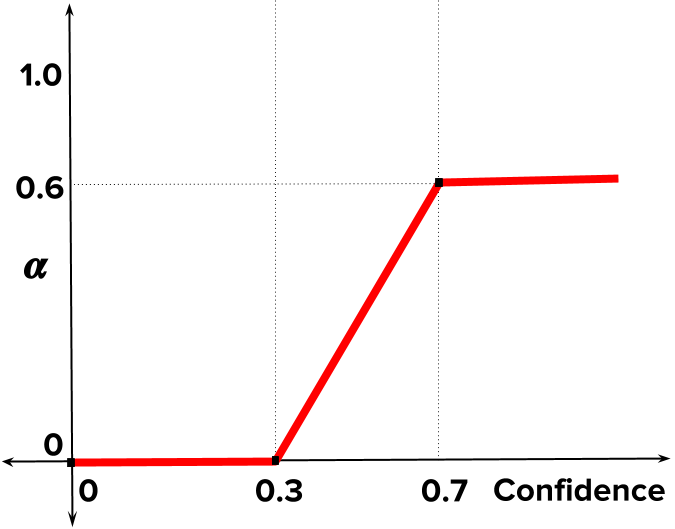
\includegraphics[width=0.2\textwidth]{./figures/ArbFunc_New1.png}
	\end{center}
	\vspace{-.3cm}
	\caption{A prototypical arbitration function.}
	\label{ALPHA}
\end{wrapfigure}
\begin{figure*}[ht]
	\centering
	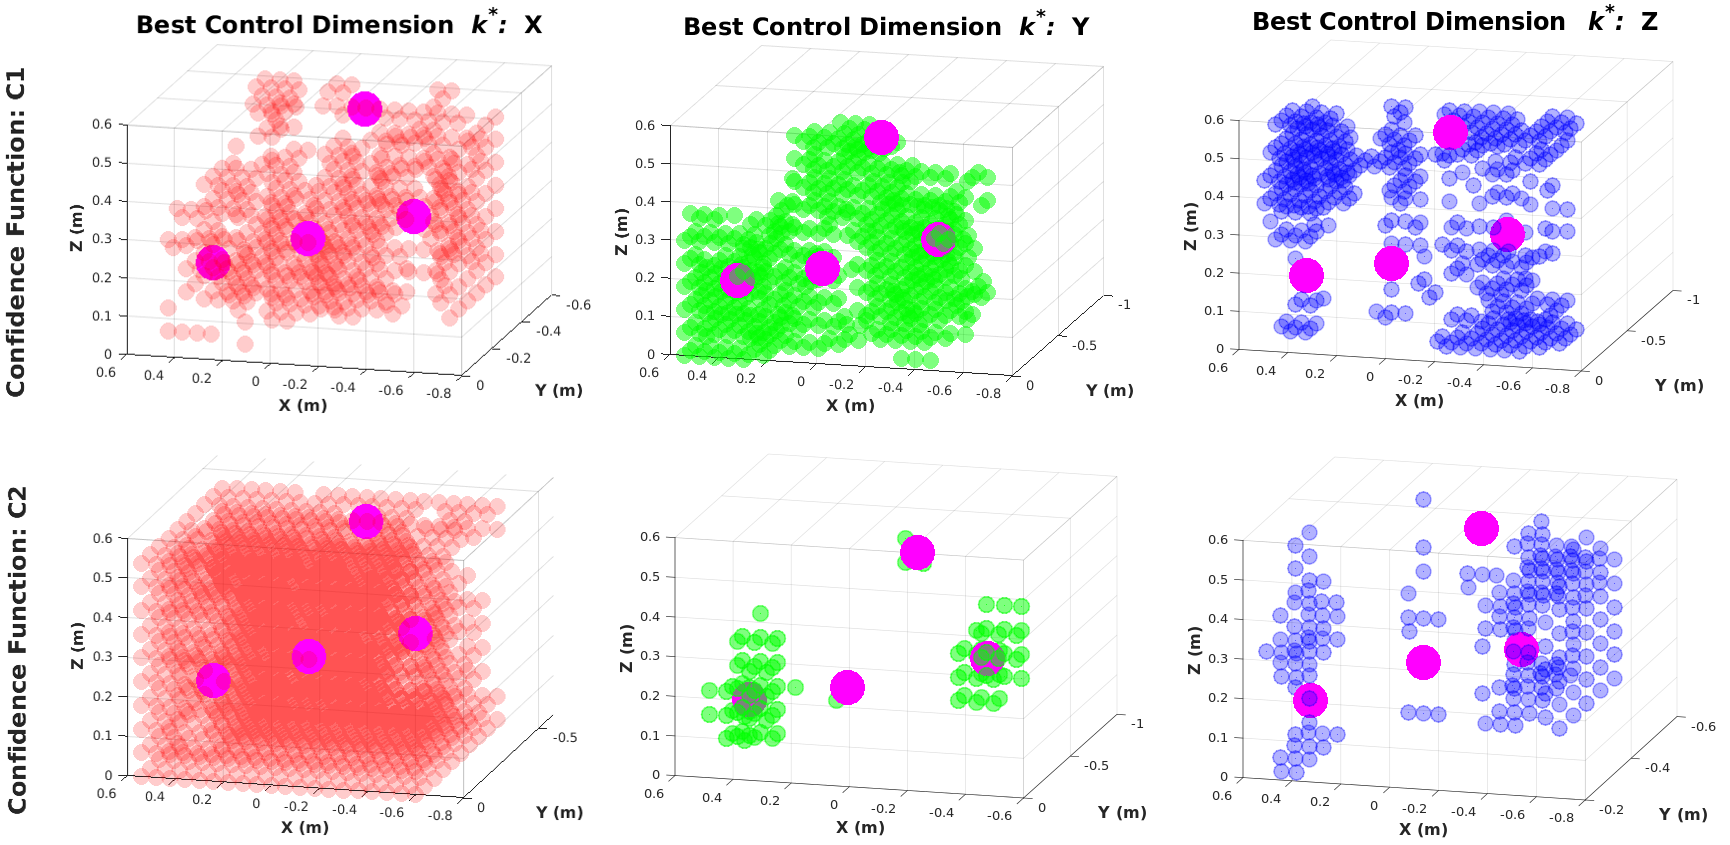
\includegraphics[width = 1\hsize, height = 0.35\vsize]{./figures/POINT_CLOUD.png}
	\caption{Control dimensions best able to disambiguate intent. Using confidence functions \textbf{C1} (top row) and \textbf{C2} (bottom row). Left column: $k^*$ is X. Middle Column: $k^*$ is Y. Right Column: $k^*$ is Z. Magenta spheres indicate the goal locations (intent).}
	\label{HM_SEP}
\end{figure*}
In our implementation, the proposed disambiguation assistance paradigm augments a blending-based shared control system, in which the final control command issued to the robot is a blended sum of the human control command and an autonomous robot policy. 
The control signal from the robot autonomy is generated by a function $f_{r}(\cdot) \in \mathcal{F}_{r}$, 
\begin{equation*}
\boldsymbol{u}_r \leftarrow f_{r}(\boldsymbol{x})
\end{equation*}
where $\mathcal{F}_{r}$ is the set of all control behaviors corresponding to different tasks.
Specifically, let $\boldsymbol{u}_{r,g}$ be the autonomous control policy associated with goal $g$. The final control command $\boldsymbol{u}$, issued to the robot then \textcolor{blue}{is} given as 
\begin{equation*}
\boldsymbol{u} = \alpha\cdot \boldsymbol{u}_{r,g^*} + (1 - \alpha)\cdot \boldsymbol{u}_h
\end{equation*}
where $g^*$ is the most confident goal. The blending factor $\alpha$ is a function of the system's confidence (Figure~\ref{ALPHA}).

The robot control command $\boldsymbol{u}_{r,g}$ is generated using a simple potential field based dynamical system which is defined in all parts of the state space. In our implementation, each goal is a position in space ($\boldsymbol{x}_g$). Every goal $g$ is associated with a potential field $P_g$ which treats $g$ as an attractor and all the other goals in the scene as repellers. For potential field $P_g$, the attractor velocity is given by
\begin{equation*}
\dot{\boldsymbol{x}}_{attract} = \boldsymbol{x}_{g} - \boldsymbol{x}
\end{equation*}
where $\boldsymbol{x}_{g}$ is the location of $g$. The repeller velocity is given by
\begin{equation*}
\dot{\boldsymbol{x}}_{repel} = \sum_{i \in \mathcal{G} \setminus g} \frac{\boldsymbol{x} - \boldsymbol{x}_{i}}{\eta(\norm{\boldsymbol{x} - \boldsymbol{x}_{i}}^2)}
\end{equation*}
where $\dot{\boldsymbol{x}}$ indicates the velocity of the robot in the world frame and $\eta$ controls the magnitude of the repeller velocity. Therefore, 
\begin{equation*}
\boldsymbol{u}_{r,g} = \dot{\boldsymbol{x}}_{attract} + \dot{\boldsymbol{x}}_{repel} 
\end{equation*}
Additionally, $P_g$ operates in the full six dimensional Cartesian space and treats position and orientation as independent potential fields. 

\section{SIMULATION ANALYSIS} \label{SIMRESULTS}
\textcolor{blue}{In this section we qualitatively look at whether our disambiguation algorithm selects modes that are intuitive and useful for intent disambiguation for a given goal configuration. We also evaluate the impact of certain simplification assumptions in our algorithm and of the choice of confidence functions within a simulated environment.}

\subsection{Choice of Confidence Functions}
\textcolor{blue}{The choice of confidence functions can greatly affect the computation of $k^*$ and $m^*$. In order to quantify the disambiguating power of different choices of confidence function, we perform simulations in which $k^*$ is computed at $2000$ uniformly sampled points in the workspace of the robotic arm (a simulated version of the robotic arm described in Section~\ref{HARDWARE}), approximated as a $1.2\times0.6\times0.7 m^3$ volume in front of the robot. Confidence functions \textbf{C1} ($r=0.3m$) and \textbf{C2}, are evaluated and the goal configuration was the same as in Figure~\ref{TASKS} (middle column). Since the target orientations are the same for all goals, disambiguation only happened in the translational dimensions and therefore is reduced to a three-dimensional problem.}

Figure~\ref{HM_SEP} shows the results of the simulation. It is clear that the choice of confidence function changes the preferred control dimension in the workspace quite significantly. Table~\ref{HMD} also reports the number of times the algorithm picked each of the three control dimensions, for each confidence function.

\textcolor{blue}{These results also shed light on the efficacy of a confidence function in properly capturing human intent}. For the goal distribution used in the simulation, the goal positions are spread out maximally along the $x$ and $z$ axes. Intuitively the system will be able to quickly infer the human's intent if the human control command is either along the $x$ or the $z$ axes. 

\textcolor{blue}{However, under confidence function \textbf{C1} the information is equally spread throughout all control dimensions (Table~\ref{HMD})---because \textbf{C1} contains less information content with respect to the user's selected motion and therefore also their intended goal. Furthermore, \textbf{C1} had ``null'' spaces where all confidences are identically equal to zero and therefore neither disambiguation nor intent inference are possible.}
\begin{table}[t]
	\centering
	\begin{tabular}{|c|c|c|c|c|}
		\hline
		\multicolumn{5}{|c|}{Best control dimension distribution} \\
		\hline
		\textbf{Confidence Function} & \textbf{X} & \textbf{Y} & \textbf{Z} & \textbf{NULL} \\ \hline
		
		\textbf{C1} & $579$ & $615$ & $446$ & $360$ \\ \hline
		\textbf{C2} & $1711$ & $93$ & $196$ & $0$\\ \hline
		
	\end{tabular}
	\vspace{.2cm}
	\caption{Best control dimension distribution for two different confidence functions.} 
	\label{HMD}
	\vspace{-.5cm}
\end{table}

\textcolor{blue}{By contrast, using \textbf{C2},  $x$ is identified as the preferred dimension in 1711 out of 2000 samples, and $z$ in 196 of the remaining 289 samples, which indicates that the confidence function along with our algorithm is able to select the disambiguating dimensions over $95\%$ of the time. The algorithm picked $y$ only when the robot is directly in front of a goal.}
\begin{table}[b]
	\centering
	\begin{tabular}{|c|c|c|c|}
		\hline
		$n_g$ & 3 & 4 & 5 \\
		\hline
		Accuracy\% & 89.24 & 87.09 & 86.11 \\
		\hline
	\end{tabular}
	\vspace{.2cm}
	\caption{Disambiguation accuracy for off-axis motions} 
	\label{SIM}
	\vspace{-.5cm}
\end{table}
\subsection{Characterization of Simplifying Assumption}
In our algorithm, the computation of $D_{m}$ only considers motion projected along perpendicular vectors: the axes of each dimension $k^i$ of mode $m$. However, in reality the user can generate a control command in any arbitrary direction within the control mode, and so the robot can move along any vector spanned by the control dimensions in $m$. In order to assess the impact of this simplification, we performed simulations in which $m^*$ was computed for $500$ uniformly spaced locations in the robot workspace. At each of those points, $100$ random control commands feasible in $m^*$ were generated and applied to perturb the robot. Finally, at each of these perturbed positions the best control mode was once again computed. 

\textcolor{blue}{If the best mode in the perturbed position was indeed mode $m^*$, then the simplification did not adversely affect the identification of the disambiguating mode. Table~\ref{SIM} summarizes the number of times a match occurred for different configurations of the workspace (with $n_g$ = $3,4$ and $5$). While the simplification does hold for $85$-$90\%$ of off-axis motions, we also do observe a trend where performance drops as the number of goals increases. Intuitively this makes sense because disambiguation between goals will become harder with a larger number of goals.}
 
 \subsection{Discussion}
Our simulation results indicate a strong correlation between the intent inference power of a given confidence function and the disambiguation power of our algorithm. It is unsurprising that confidence functions which are information-poor approximations of human intent also perform less robustly when disambiguating between those approximations.
 Moreover, the algorithm could be used to pre-compute the most informative modes ahead of time, which then might be called on-demand during the task execution---which could prove helpful for complex tasks and/or limited interfaces that require more information from the human for disambiguation. 
 \section{PILOT STUDY} \label{EXP}
 We next explore the use and utility of our disambiguation approach in a pilot study. Four subjects participated in the pilot study (3 male, 1 female), and all were lab members.
 \subsection{Hardware}\label{HARDWARE}
 

\begin{figure}[h]
	\centering
	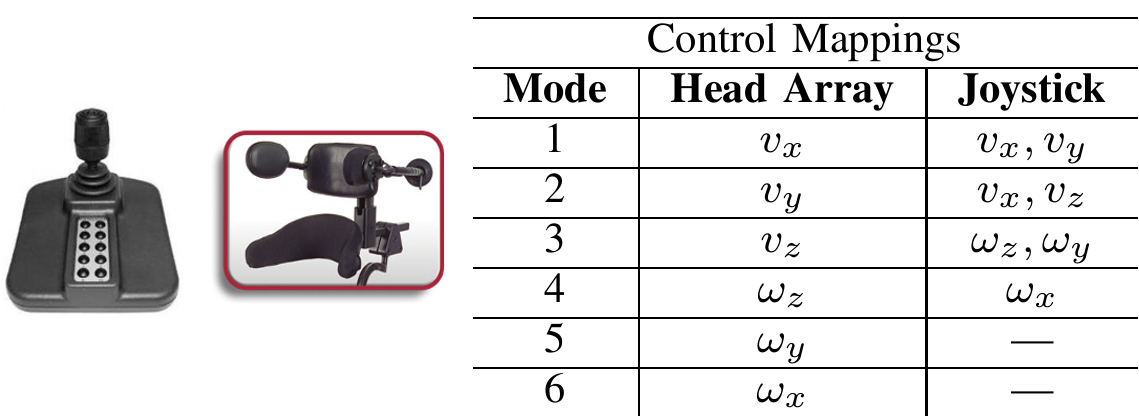
\includegraphics[width = 1\hsize, height = 0.14\vsize]{./figures/INTER_3.png}
	\vspace{-0.3cm}
	\caption{A 2-axis joystick (left) and switch-based head array (center) and their operational paradigms (right). $v$ and $\omega$ indicate the translational and rotational velocities of the end-effector, respectively.}
	\label{J2_HA}
\end{figure}
\begin{figure*}[ht]
	\centering
	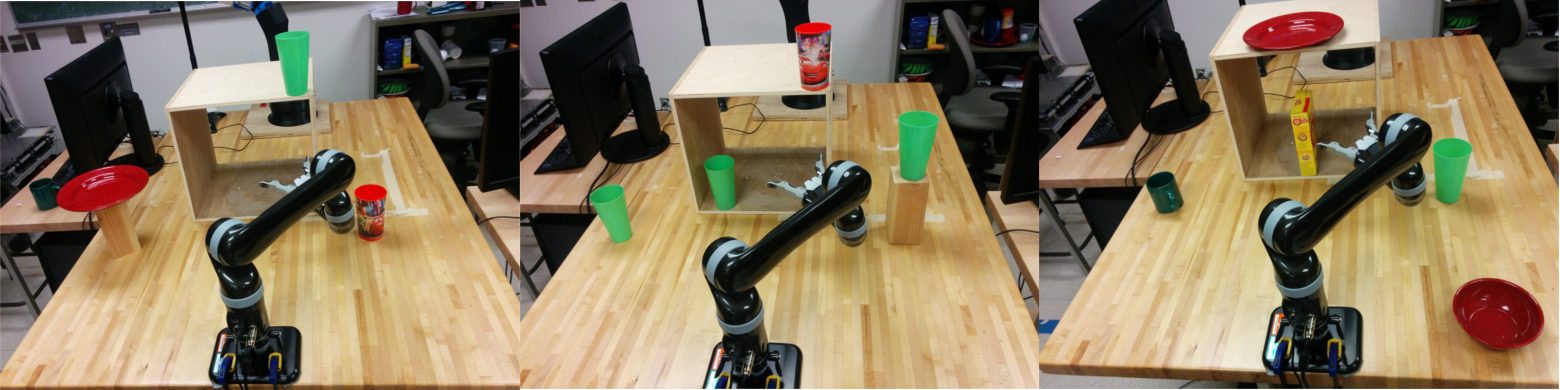
\includegraphics[width = 1\hsize]{./figures/TASKS.png}
	\caption{Pilot study tasks. \textit{Left to right:} Training, Testing (Easy), Testing (Hard).}
	\label{TASKS}
\end{figure*}
 The experiments were performed using the MICO robotic arm (Kinova Robotics, Canada), which is a 6-DoF robotic arm specifically designed for assistive purposes. The software system was implemented using the Robot Operating System (ROS) and data analysis was performed using MATLAB.\footnote{Additionally, for the 6-D robot arm implementation, the computation of \textbf{C2} is split into translational and rotational components. (In Section~\ref{SIMRESULTS}, only translational components were considered.) Here confidence function \textbf{C2} is computed as
 	$c(\boldsymbol{x}, \boldsymbol{u}_h, \boldsymbol{u}_{r,g}) = \boldsymbol{u}_{h}^{trans}\cdot(\boldsymbol{x}_{g} - \boldsymbol{x})^{trans} + \boldsymbol{u}_h^{rot}\cdot\boldsymbol{u}_{r,g}^{(rot)}$
 	where $trans$ refers to the translational and $rot$ the rotational parts of the full control space.}
 
 \textcolor{blue}{The human control command $\boldsymbol{u}_h$ was captured using two different control interfaces: 2-axis joystick and a 1-D head array, shown in Figure~\ref{J2_HA}. For both interfaces, the control interface signals were mapped to Cartesian velocities of the end-effector of the robot. Additionally, the interfaces were used to request mode switch assistance.}
 
 \textcolor{blue}{In detail, the joystick generated continuous signals and was capable of controlling a maximum of two control dimensions at a time. Different control modes could be accessed using the buttons on the interface. 
 The head array generated 1-D discrete control signals, and consisted of three switches operated by the head and embedded within the back and sides of the headrest. When used for controlling a robotic arm, the switch at the back was used to cycle between the control modes, and the switches on the left and right sides controlled the motion of the end-effector in positive and negative directions along the control dimension of the selected control mode. In using two interfaces, our aim was to observe whether differences in interface dimensionality and continuity correlated with any differences in task performance and mode switching.}
 
 \subsection{\textcolor{blue}{Assistance Paradigms}}
 Three kinds of mode switching paradigms were evaluated. Note that the blending assistance (as described in Section~\ref{BP}) was always running for all three paradigms. Since under the blending paradigm the amount of assistance directly depended on the amount of confidence, this meant that if the intent inference improved as a result of disambiguation, more assistance would be provided by the robot.
 
 \noindent\underline{\textit{Manual}}: The trial started in a randomized initial mode and during task execution the user manually performed all subsequent mode switches.
 
 \noindent\underline{\textit{Disambiguation}}: The disambiguation system was activated right at the beginning of a trial. The algorithm identified the ``best mode'' $m^*$ and started the trial in mode $m^*$. All subsequent mode switches were performed manually by the user. Furthermore, the user was required to first move in the selected mode before manually switching the mode. 
 
 \noindent\underline{\textit{On-Demand}}: The user could request mode switch assistance at any time during the task execution. This paradigm was exploratory and sought to find underlying patterns in assistance request behavior.
 
\subsection{\textcolor{blue}{Tasks, Metrics and Protocol}}

\noindent\underline{\textit{Tasks}}: Training and Testing tasks were developed for the pilot study (Figure~\ref{TASKS}). \textbf{Training}: The user operated the robotic arm to perform simple reaching motions to three different goal locations. The primary purpose was to get the user accustomed to the operation of the interfaces, the blending-based assistance and the experiment protocol. \textbf{Testing}: The user operated the robotic arm under two scenarios of varying difficulty. \textit{Easy}: Four objects, all with the same grasp orientations. \textit{Hard}: Five objects, all with different grasp orientations.

\noindent\underline{\textit{Metrics}}: \textit{Task completion time} is the amount of time a user spent in accomplishing a task. \textit{Mode switches} refers to the number of times the user switched between various modes while performing the task. 

\noindent\underline{\textit{Protocol}}: A within-subjects study was conducted using a full factorial design in which the manipulated variables were the tasks, control interfaces and assistance paradigms. Each task consisted of two phases. 

In Phase I, each user performed the task using both interfaces under the \textit{Manual} and \textit{Disambiguation} paradigms. The trials were balanced and the control interfaces and the paradigms were randomized to eliminate ordering effects. The starting positions of the robot also were randomized to avoid biases. Three trials were collected for each permutation of manipulated variables. 
In Phase II, the user performed the same task using both interfaces and the \textit{On-Demand} paradigm, and two trials were collected for each task-interface combination.  

\subsection{Pilot Study Results}\label{RES}
An improvement in task performance in terms of a decrease in the number of mode switches was observed across both interfaces. Statistical significance in Figure~\ref{DATAPLOT} was determined by a two-sided Wilcoxon Rank-Sum Test, where (*) indicates $p < 0.05$ and (***) indicates $p < 0.001$.

\begin{figure}[t]
	\centering
	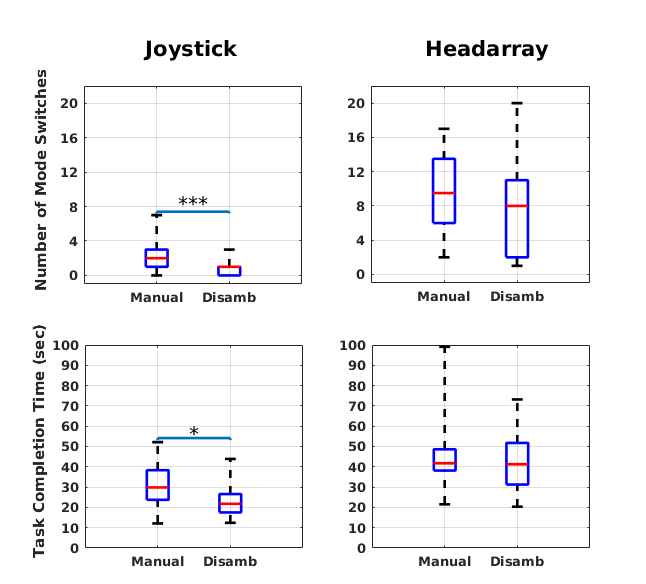
\includegraphics[width = 1.11\hsize ,center]{./figures/FINAL_BOXPLOT_3.png}
	\vspace{-0.7cm}
	\caption{Comparison of Disambiguation and Manual paradigms. Operation using joystick (left column) and head array (right column) interfaces. Evaluation of mode switches (top row) and completion time (bottom row). \textcolor{blue}{Box plots show the median and the quartiles}.}
	\label{DATAPLOT}
\end{figure}
\vspace{0.1cm}
\noindent{\underline{\textit{Mode Switches}}}: Figure~\ref{DATAPLOT} (top row) reveals a general trend of a decrease in the number of mode switches when disambiguation assistance was employed. This indicates that upon starting in a mode identified by the algorithm, the number of subsequent mode switches performed by the user was reduced.
 
\textcolor{blue}{Somewhat surprisingly, this difference in number of mode switches was significant only when using the joystick. The head array moreover required more mode switches to complete the task. We also observe a much larger spread across trials and users.}

\vspace{0.1cm}
\textcolor{blue}{\noindent{\underline{\textit{Task Completion Time}}}: 
In Figure~\ref{DATAPLOT} (bottom row), a statistically significant decrease in task completion times between the \textit{Manual} and \textit{Disambiguation} paradigms was observed when using the joystick. The task completion times were comparable between the two paradigms when using the head array. }

\textcolor{blue}{This difference in task success might be explained by the fact that a \textit{single} mode switch assistance at the beginning of the trial probably did not have a measurable impact in reducing the subsequent number of mode switches needed when using a head array---which required many more mode switches to achieve a task (Figure~\ref{DATAPLOT}, top row). Such a conclusion would have a utility implication for our algorithm---that as the number of required mode switches increases, so too must the number of disambiguation operations if disambiguation assistance is to be used.}

\vspace{0.1cm}
\noindent{\underline{\textit{On-Demand}}}: The number of disambiguation requests under the \textit{On-Demand} paradigm are reported in Table~\ref{ONDEMAND}. Although the subjects demonstrated a wide range of disambiguation request behaviors, we are able to observe a general trend of an increase in disambiguation requests with an increase in task difficulty. This shows that users were keen to explore the \textit{On-Demand} option when the tasks became more difficult. 

\subsection{Future Work}
\textcolor{blue}{Post-experiment feedback from the users also revealed that the subjects found the disambiguation assistance to be counter-intuitive at times in the \textit{On-Demand} paradigm. This might be attributable to two main limitations of the current algorithm.}

\textcolor{blue}{First, when the user requests assistance (in the \textit{On-Demand} paradigm) at any point in time and space, the algorithm discards all information contained in the history of user commands from the start of the trial until that point. That is, the disambiguation algorithm lacks \textit{memory} and reasons about the user's intent solely based on information that is available locally. However, it might be useful to bias the computation of the disambiguating control mode by incorporating information from the past history of the robot trajectory and control commands, by having a non-uniform prior over the intended goals. This would also likely improve the robustness and efficacy of the algorithm, and result in higher user acceptance.}

\textcolor{blue}{Second, the algorithm only tries to maximize the utility value \textit{for} the robot. However, it also is important to take into account the user's preference and ability to operate in the mode selected by the algorithm. Concepts from decision theory might be used to enhance the current framework.}

Our pilot study revealed some promising trends and therefore a more extensive user study with motor-impaired subjects will be conducted in the future, to evaluate the utility of the disambiguation assistance system and further explore and understand the disambiguation request patterns of users.
\section{CONCLUSIONS}\label{DC}
\begin{table}[t]
	\centering
	\begin{tabular}{ccccc}
		\toprule
		&\multicolumn{2}{c}{Joystick}
		&
		\multicolumn{2}{c}{Head Array} \\\cmidrule(r){2-3}\cmidrule(l){4-5}
		Subject &\textit{Easy}& \textit{Hard}    & \textit{Easy} &\textit{Hard}      \\
		\bottomrule
		1 &1& 0   & 5 & 6  \\
		\bottomrule
		2 &1& 1    & 3 & 6      \\
		\bottomrule
		3 &2& 2    & 4 &5    \\
		\bottomrule
		4 &2& 5    & 17 &7   \\
		\bottomrule
	\end{tabular}
	\vspace{.2cm}
	\caption{Number of Disambiguation requests}
	%\vspace{-0.2cm}
	\label{ONDEMAND}
\end{table}
In this paper, we have presented an algorithm for \textit{intent disambiguation assistance} with a shared-control robotic arm. We also introduced the notion of \textit{inverse legibility}, in which the human-generated actions are legible enough \textit{for} the robot to infer the human intent confidently and accurately. The goal of the algorithm developed in this paper is to seek legible control commands from the human by placing control in those modes able to \textit{maximally disambiguate} between various goals. Preliminary pilot study results suggested that the proposed disambiguation paradigm to be promising. \textcolor{blue}{Our simulation work evaluated the impact of the simplifying assumptions and of different confidence functions on intent disambiguation.} In our future work, as informed by the pilot study, we plan to enhance the algorithm and extend the framework into an automated mode switch assistance system. 

\section*{Acknowledgments}
This material is based upon work supported by the National Science Foundation under Grant CNS 15544741. Any opinions, findings and conclusions or
recommendations expressed in this material are those of the authors and do
not necessarily reflect the views of the aforementioned institutions.
%Funding source omitted for review. 
%\subsection{Subsection Heading Here}
%Subsection text here.
%
%\subsubsection{Subsubsection Heading Here}

%
%
%\section{RSS citations}
%
%Please make sure to include \verb!natbib.sty! and to use the
%\verb!plainnat.bst! bibliography style. \verb!natbib! provides additional
%citation commands, most usefully \verb!\citet!. For example, rather than the
%awkward construction 
%
%{\small
%\begin{verbatim}
%\cite{kalman1960new} demonstrated...
%\end{verbatim}
%}
%
%\noindent
%rendered as ``\cite{kalman1960new} demonstrated...,''
%or the
%inconvenient 
%
%{\small
%\begin{verbatim}
%Kalman \cite{kalman1960new} 
%demonstrated...
%\end{verbatim}
%}
%
%\noindent
%rendered as 
%``Kalman \cite{kalman1960new} demonstrated...'', 
%one can
%write 
%
%{\small
%\begin{verbatim}
%\citet{kalman1960new} demonstrated... 
%\end{verbatim}
%}
%\noindent
%which renders as ``\citet{kalman1960new} demonstrated...'' and is 
%both easy to write and much easier to read.
%  
%\subsection{RSS Hyperlinks}
%
%This year, we would like to use the ability of PDF viewers to interpret
%hyperlinks, specifically to allow each reference in the bibliography to be a
%link to an online version of the reference. 
%As an example, if you were to cite ``Passive Dynamic Walking''
%\cite{McGeer01041990}, the entry in the bibtex would read:
%
%{\small
%\begin{verbatim}
%@article{McGeer01041990,
%  author = {McGeer, Tad}, 
%  title = {\href{http://ijr.sagepub.com/content/9/2/62.abstract}{Passive Dynamic Walking}}, 
%  volume = {9}, 
%  number = {2}, 
%  pages = {62-82}, 
%  year = {1990}, 
%  doi = {10.1177/027836499000900206}, 
%  URL = {http://ijr.sagepub.com/content/9/2/62.abstract}, 
%  eprint = {http://ijr.sagepub.com/content/9/2/62.full.pdf+html}, 
%  journal = {The International Journal of Robotics Research}
%}
%\end{verbatim}
%}
%\noindent
%and the entry in the compiled PDF would look like:
%
%\def\tmplabel#1{[#1]}
%
%\begin{enumerate}
%\item[\tmplabel{1}] Tad McGeer. \href{http://ijr.sagepub.com/content/9/2/62.abstract}{Passive Dynamic
%Walking}. {\em The International Journal of Robotics Research}, 9(2):62--82,
%1990.
%\end{enumerate}
%%
%where the title of the article is a link that takes you to the article on IJRR's website. 
%
%
%Linking cited articles will not always be possible, especially for
%older articles. There are also often several versions of papers
%online: authors are free to decide what to use as the link destination
%yet we strongly encourage to link to archival or publisher sites
%(such as IEEE Xplore or Sage Journals).  We encourage all authors to use this feature to
%the extent possible.
%
%\section{Conclusion} 
%\label{sec:conclusion}
%
%The conclusion goes here.

%\section*{Acknowledgments}

%% Use plainnat to work nicely with natbib. 

\bibliographystyle{plainnat}
\bibliography{references}

\end{document}


